\chapter{Zukünftige Entwicklungsmöglichkeiten}
Obwohl das Praktikum ein voller Erfolg war werden in diesem Kapitel noch Verbesserungsvorschläge und Ausbaumöglichkeiten beleuchtet. 

\section{Regler}
Die Messwerte des Gyroskops können für einen Regelkreis (Abb.~\ref{bild:regler}) benutzt werden. 

\begin{figure}[!ht]
	\centering
	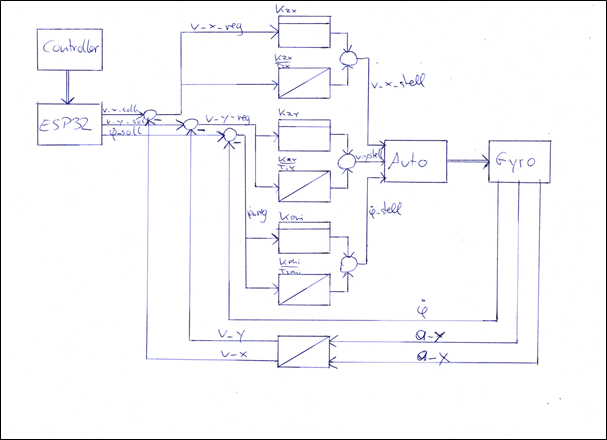
\includegraphics[width=\textwidth]{bilder/regler.png}
	\caption{Blockschaltbild Regler}
	\label{bild:regler}
\end{figure}

Durch die Eingaben des Spiele-Controllers und deren Interpretation durch das ESP-32 werden Sollwerte für Geschwindigkeiten in allen Achsen vorgegeben. 
Das Gyroskop misst Beschleunigung in X- und Y-Richtung und die Winkelgeschwindigkeit der Rotation. 

Deswegen müssen die Beschleunigungswerte einmal integriert werden, um auf die momentane Ist-Geschwindigkeit in beiden Richtungen zu kommen. 
Das übernimmt der Integrator ganz unten. 

Anschließend wird von den Soll- und Ist-Werten die Differenz gebildet. 
Über diese Regelungsdifferenz wird jeweils durch einen PI-Regler (Proportional und Integrationsglied) mit empirisch bestimmten Faktoren die Stellgröße ermittelt. 
Das Integrationsglied der PI-Regler ist dabei wichtig für die stationäre Genauigkeit. 

Die Stellgrößen werden nach Umrechnung an die Motoren weitergeleitet, was wiederum zu veränderten Messgrößen am Gyroskop führt. 
Damit ist der Kreis geschlossen. 


\section{Verbesserungen}
\subsection{Hardware}

\subsection{Software}
